\begin{center}\rule{0.5\linewidth}{0.5pt}\end{center}

\subsection{Discriminator and Generator
Losses}\label{discriminator-and-generator-losses}

Now we need to calculate the losses.

\subsubsection{Discriminator Losses}\label{discriminator-losses}

\begin{quote}
\begin{itemize}
\item For the discriminator, the total loss is the sum of the losses for
  real and fake images,
  \lstinline{d_loss = d_real_loss + d_fake_loss}.
\item  Remember that we want the discriminator to output 1 for real images
  and 0 for fake images, so we need to set up the losses to reflect
  that.
\end{itemize}
\end{quote}

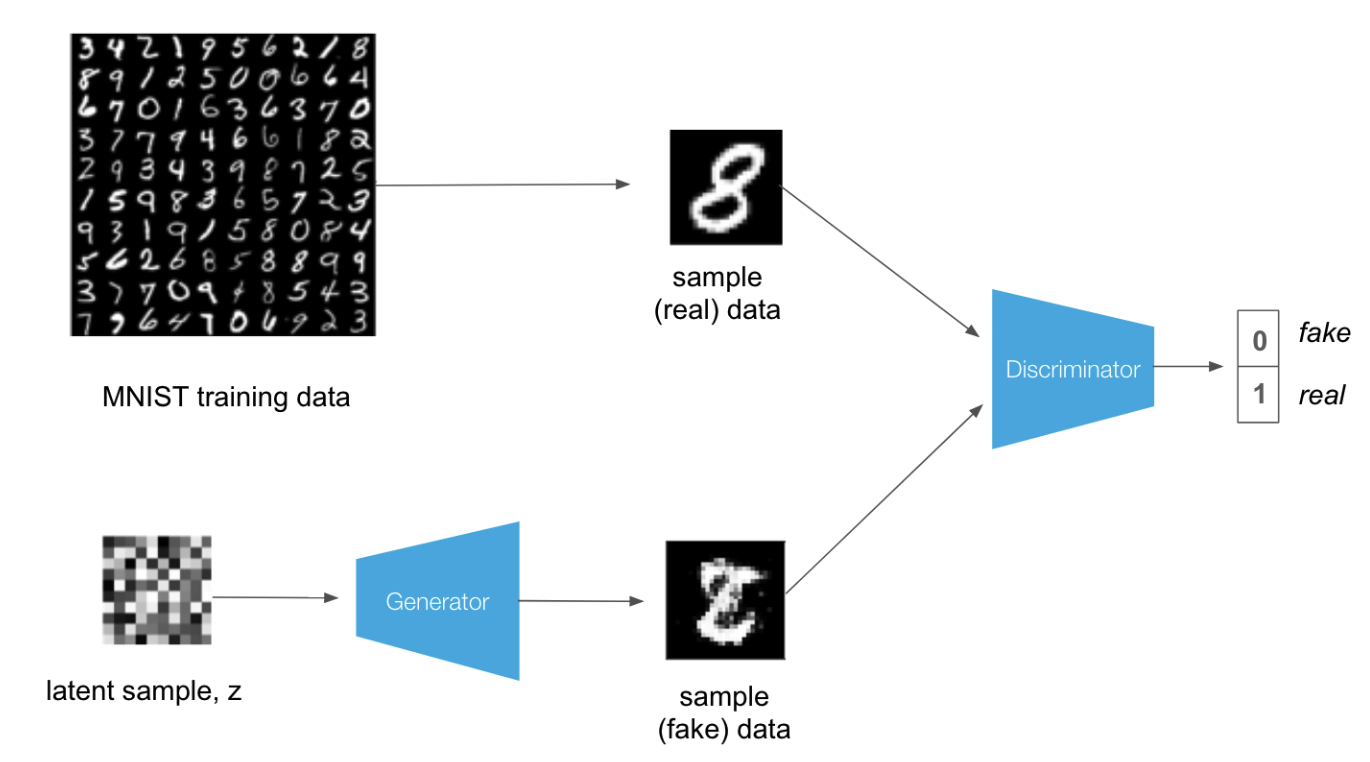
\includegraphics[width=1\linewidth]{img//genAdvNet//gan/part2_screengrab.png}

The losses will by binary cross entropy loss with logits, which we can
get with
\href{https://pytorch.org/docs/stable/nn.html\#bcewithlogitsloss}{BCEWithLogitsLoss}.
This combines a \lstinline{sigmoid} activation function
\textbf{and} and binary cross entropy loss in one function.\newline

For the real images, we want
\lstinline{D(real_images) = 1}. That is, we want the
discriminator to classify the the real images with a label = 1,
indicating that these are real. To help the discriminator generalize
better, the labels are \textbf{reduced a bit from 1.0 to 0.9}. For this,
we'll use the parameter \lstinline{smooth}; if True, then
we should smooth our labels by a factor of 0.9 .\newline

The discriminator loss for the fake data is similar. We want
\lstinline{D(fake_images) = 0}, where the fake images are
the \emph{generator output},
\lstinline{fake_images = G(z)}.

\begin{lstlisting}[language=Python]
import torch
import torch.nn as nn

import tests
\end{lstlisting}

\begin{lstlisting}[language=Python]
# Calculate losses
def real_loss(D_out, smooth=False):
    if smooth:
        labels = torch.ones_like(D_out) * 0.9
    else:
        labels = torch.ones_like(D_out)
    
    criterion = nn.BCEWithLogitsLoss()
    
    loss = criterion(D_out, labels)
    return loss
\end{lstlisting}

\begin{lstlisting}[language=Python]
tests.check_real_loss(real_loss)
\end{lstlisting}

\begin{lstlisting}
Congrats, you successfully implemented the real loss function
Congrats, you successfully implemented the real loss function with smoothing
\end{lstlisting}

\subsubsection{Generator Loss}\label{generator-loss}

The generator loss will look similar only with flipped labels. The
generator's goal is to get
\lstinline{D(fake_images) = 1}. In this case, the labels
are \textbf{flipped} to represent that the generator is trying to fool
the discriminator into thinking that the images it generates (fakes) are
real!

\begin{lstlisting}[language=Python]
def fake_loss(D_out):
    labels = torch.zeros_like(D_out)
    
    criterion = nn.BCEWithLogitsLoss()
    
    loss = criterion(D_out, labels)
    return loss
\end{lstlisting}

\begin{lstlisting}[language=Python]
tests.check_fake_loss(fake_loss)
\end{lstlisting}

\begin{lstlisting}
Congrats, you successfully implemented the fake loss function
\end{lstlisting}
